\documentclass[10pt,a4paper]{article}
\usepackage[utf8]{inputenc}
\usepackage{amsmath}
\usepackage{amsfonts}
\usepackage{amssymb}
\usepackage{fullpage}
\usepackage{verbatim}
\usepackage{graphicx}

\usepackage{subcaption}
\begin{document}

\title{Towards detecting critical crowd density with Wi-Fi positioning: Case Amsterdam ArenA}
\author{Sonja Georgievska, Philip Rutten, Jan Amoraal, Michael Lees, Sander Klous\footnote{authors and order could change by the time the paper is submitted}}
\maketitle

\begin{abstract}

We present a new methodology for estimating crowd density during festivals. Our motivation comes from the fact that many crowd disasters have happened because of abnormal crowd density. We exploit the ubiquity of smart phones, without requiring participation from the crowd, and we use Amsterdam ArenA as a living laboratory. We build upon previous work, where the location of a visitor is estimated anonymously based on the strengths of the Wi-Fi signals received at the ArenA Wi-Fi routers,  by a method similar to trilateration. However, because in dense crowds a Wi-Fi signal is partially absorbed and partially reflected by the human bodies, the localization based on signals strengths alone does not suffice to estimate the crowd density. Moreover, since we don't rely on the smart phones being connected to the Wi-Fi network, the signal rates are quite volatile, and the MAC addresses of the phones may change, depending on the vendor's privacy policy. In this paper, we address those issues. We borrow ideas from statistical mechanics to estimate the crowd density. \begin{comment} rather than estimating the position of a visitor, we create a continuous probability distribution over all possible positions. We rely on the law of the large numbers, with adaptation to correlated variables, to estimate the crowd density by aggregating the individual distributions. The individual probability distribution turns gradually into a uniform distribution, with which we address the problem of outdated signals. Finally, we use the law of large numbers again and the "randomized address" tag to account for the fact that a portion of the MAC addresses are randomized. Thus, \end{comment} 
The advantage of our methodology when compared to similar methodologies is that our estimation becomes more (rather than less) precise when the number of people increases. This suits the purpose of being able to detect raised crowd density. 
We also validate our methodology experimentally by comparing the crowd density estimation to the ground truth obtained from security cameras. \marginpar{val. to be done}
	
\begin{comment} From Philip:
We present the Amsterdam Arena project, which involves observing and managing crowd behaviour, using the Amsterdam Arena stadium as a living laboratory. The main scientific question we explore is how to detect anomalous behaviour in large crowds in real time. The main purpose is to be able to predict a possible crowd disaster and identify means to prevent it from happening. 
Human crowds are complex systems, and predicting or controlling their behaviour is challenging. Our approach involves three phases, firstly data collection from Wi-Fi and Bluetooth sensors in the stadium, secondly data analytics, and finally we aim to use simulation to make forecasts about the crowd dynamics. 
Here we present initial results on the data analytics and show how we can extract density maps from Wi-Fi positioning data. The technology we deploy is based on the Wi-Fi signals from smart phones. We use the existing network of Wi-Fi access points in the stadium, and capture probe signals from smart phones, which are processed and anonymised in alignment with privacy concerns. The positions of smart phones are reconstructed using received signal strengths and methods similar to trilateration. The data provides us with real-time information on spatial distributions of crowd density, which is an essential indicator of the criticality of crowd conditions. To visualise the spatiotemporal behaviour of crowd density in real-time we dynamically generate heat maps along a moving time interval. The heat maps are generated through the statistical modelling of the positioning data. The generation of dynamic heat maps allows us to detect and locate hot-spots of density where crowd conditions reach critical values that could possibly lead to a disaster.
\end{comment}
\end{abstract}

\section{Introduction}


Crowd disasters have taken many human lives. The Love Parade disaster (Duisburg, 2010), the Ellis Park Stadium disaster (Johannesburg, 2001), the PhilSports Stadium stampede (Manila, 2006) are just a few recent examples. One of the reasons that disasters happen is a "lack of overview of everybody" \cite{Helbing2012}, that is, a lack of macroscopic overview of the crowd. Critical crowd density  \cite{Helbing2012, density} is a contributing factor to crowd disasters. Yet, it is still challenging to determine timely when it occurs, so that a disaster can be prevented by navigating the rest of the crowd away from the congestion. 

In our work we estimate crowd density during concerts in indoor spaces. A lot of research on estimating crowd density has been done using video processing from security cameras \cite{Crowded_Scene_Analysis, Krausz2012307}. However, this approach does not suffice to detect raised crowd density. First, it is difficult to obtain macroscopic overview of the crowd. Second, 
the lighting conditions during concert hours might not be sufficient for video-based crowd analysis only. Finally, the error of video-based density estimation increases with the increase of the actual crowd density.  

In our approach, which can complement the video-based analysis, we combat the three above mentioned issues by exploiting the ubiquity of smart phones, as has been done in (citations). Contrarily to most such approaches (citations), we \marginpar{add missing citations twice} don't require participation from the crowd. Our living laboratory is the Amsterdam Arena \cite{arena}.  We build upon previous work \cite{customers_jan}, where the location of a visitor is estimated anonymously based on the strengths of the Wi-Fi signals received at the ArenA Wi-Fi routers,  by a method similar to trilateration (the way the Global Positioning System is implemented). However, because in dense crowds a Wi-Fi signal is partially absorbed and partially reflected by the human bodies, the localization based on signals strengths alone does not suffice to estimate the crowd density; e.g. multiple optimal position estimations are possible.  Moreover, since we don't rely on the smart phones being connected to the Wi-Fi network, the signal rates are quite volatile, and the MAC addresses of the phones may change (be "randomized"), complying to some  vendors' privacy policy. In this paper, we address those issues. We borrow ideas from statistical mechanics to estimate the crowd density: rather than estimating the most likely position of a visitor in real time, we create an evolving continuous probability distribution over all possible positions (which turns out to be usually bimodal). We rely on the law of the large numbers, with adaptation to correlated variables, to estimate the crowd density by aggregating the individual distributions. The individual probability distribution turns gradually into a uniform distribution, with which we address the problem of outdated signals. Finally, we use the law of large numbers again and the "randomized MAC address" tag, that is available with the data, to account for the fact that a portion of the MAC addresses are randomized. Thus, the advantage of our methodology when compared to other methodologies is that our estimation becomes more (rather than less) precise when the number of people increases. This suits the purpose of being able to detect raised crowd density. 
We also validate our methodology experimentally by comparing the crowd density estimation time series to the ground truth obtained from security cameras. \marginpar{validation to be done}

\begin{comment}
Our methodology consists of three steps.  First, we are using Wi-Fi routers in the stadium to gather the strengths of the wireless antena signals from individuals smart phones.  Second, we are estimating anonymously the positions of the visitors from the signal strengths. This technique has been presented in \cite{customers_Jan}, and is similar to trilateration, that is, the way the Global Positioning System (GPS) is implemented. However, due to signal interference and blockage in dense crowds, irregular internet packet rates, and systematic errors leading to multiple local optima, the positioning itself does not suffice to estimate the crowd density. Thus, in our third step, we aggregate the results from the positioning and apply statistical ensembling to obtain an estimation of the crowd density. 

With the first two steps, we are handling issues 1) and 2) mentioned above. With the third step, which is the main contribution of this paper, we are handling issue 3) -  that is, with our method the precision of estimation actually increases as the crowd density increases. 
\end{comment}

The rest of the paper is organized as follows. In Sec. \ref{sec:positioning} we explain the process of trilateration, that estimates the position of a Wi-Fi device based on the strength of the signals captured by the Wi-Fi routers in the stadium. In Sec. \ref{sec:density} we present our methodology for estimating in real-time the spatial density distribution of the crowd. We first identify which issues have not been resolved by the positioning in order to estimate crowd density, and which are not related to the mathematical methodology behind the positioning step. Then, we present our approach towards resolving the issues. In Sec. \ref{sec:validation} we compare our estimation of density to the one  obtained by video analysis. In Sec. \ref{sec:relatedwork} we put our approach into a perspective by comparing it to other approaches that are using the smart phones. We conclude and point to future research directions in Sec. \ref{sec:conclusion}.



\marginpar{end from Sonja}


\section{Positioning of visitors using Wi-Fi sensors and smart phones}
\label{sec:positioning}


This section will be written later, maybe with input from Jan. 

The positions of smart phones are reconstructed using methods based on lateration. 
The lateration method uses the distances between a smart phone and multiple reference points, which in this case are the existing Wi-Fi access points (APs) in the stadium.
Smart phones transmit Wi-Fi signals which are captured at the APs.
The captured Wi-Fi signals contain information about the mesaured signal strength.
Using a model for the relationship between the received signal strength (RSS) of the Wi-Fi signal and the distance between transmitter and receiver, the distance between smart phone and the AP is estimated.
The distance between the position $(x,y)$ (in two dimensions) of the mobile device and the position $(x_{i},y_{i})$ of AP $i$, given by 
\begin{equation}
r_{i}^2=(x-x_{i})^2+(y-y_{i})^2
\label{distance}
\end{equation}
The distances define circles with radius $r_{i}$ around the APs on which the transmitter may be located.
When we have at least three such circles, the position of a transmitter can be uniquely determined at the intersection of the circles \cite{kushki:1}.

The RSS value of a signal decreases when the distance between transmitter and receiver increases.
The decrease is given by a path loss model, given by the Friis equation
\begin{equation}
P_{R}=P_{T}+10\lambda\log_{10}(\frac{c}{4\pi fr})
\label{friis}
\end{equation}
where we use $\lambda=2$ (line of sight condition), $c$ is the speed of light, $f$ is 2.4 GHz, and $r$ is the distance between the mobile device and the AP.\\
The measured RSS values contain unpredictable variation due to noise, and interference such as absorption and reflection by obstacles between transmitter and receiver (shadowing and multipath effects) \cite{goldsmith}. The positions of these obstacles may change in time, in particular in the case of human bodies.
As a result, the circles in the lateration method do not intersect at a unique point, and the system of equations defined in Equation \ref{distance} do not have an exact solution.
In this case a statistical approach is taken to the determination of the position of the smart phone.
The least squares method is used, which in our case takes the form of a chi-square data fit \cite{bevington}.
Based on the chi-square fit, uncertainty values for the parameter estimates are calculated.
These values represent parameter uncertainties that correspond to a $1\sigma$ error or an increase of $\chi^2+1$. 
The $1\sigma$ error values form the input to the smoothing method of the density estimation discussed in this paper.

\begin{comment}
The technology we deploy is based on the Wi-Fi signals from smart phones. We use the existing network of Wi-Fi access points in the stadium, and capture probe signals from smart phones, which are processed and anonymised in alignment with privacy concerns. The positions of smart phones are reconstructed using received signal strength (RSS) values and methods similar to multi-lateration. 


\begin{itemize}
\item How are the uncertainties (errors) generated and what do they mean?
\end{itemize}
\end{comment}
\section{From positioning to estimation of density}
\label{sec:density}


\subsection{Positioning only is not enough}

Under ideal circumstances, the positioning itself would suffice to estimate the spatial crowd density distribution:  every second we would only need to count the number of estimates per square meter. However, we have observed several issues, which are not related to the mathematical methodology behind the positioning step, that prevent us to apply direct counting. 
\begin{enumerate}
	\item
	{\it Issue 1: bimodal distributions of coordinates estimations}. We have sampled randomly 20 MAC addresses and plotted the estimations of their coordinates through time, where we have plotted only the estimations with a relatively small (conditional) uncertainty. We observed persistent bimodal distribution of the estimations, an example of which can be seen in Fig. \ref{fig:bimodal}. 
		\begin{figure}[h!]
			\centering
			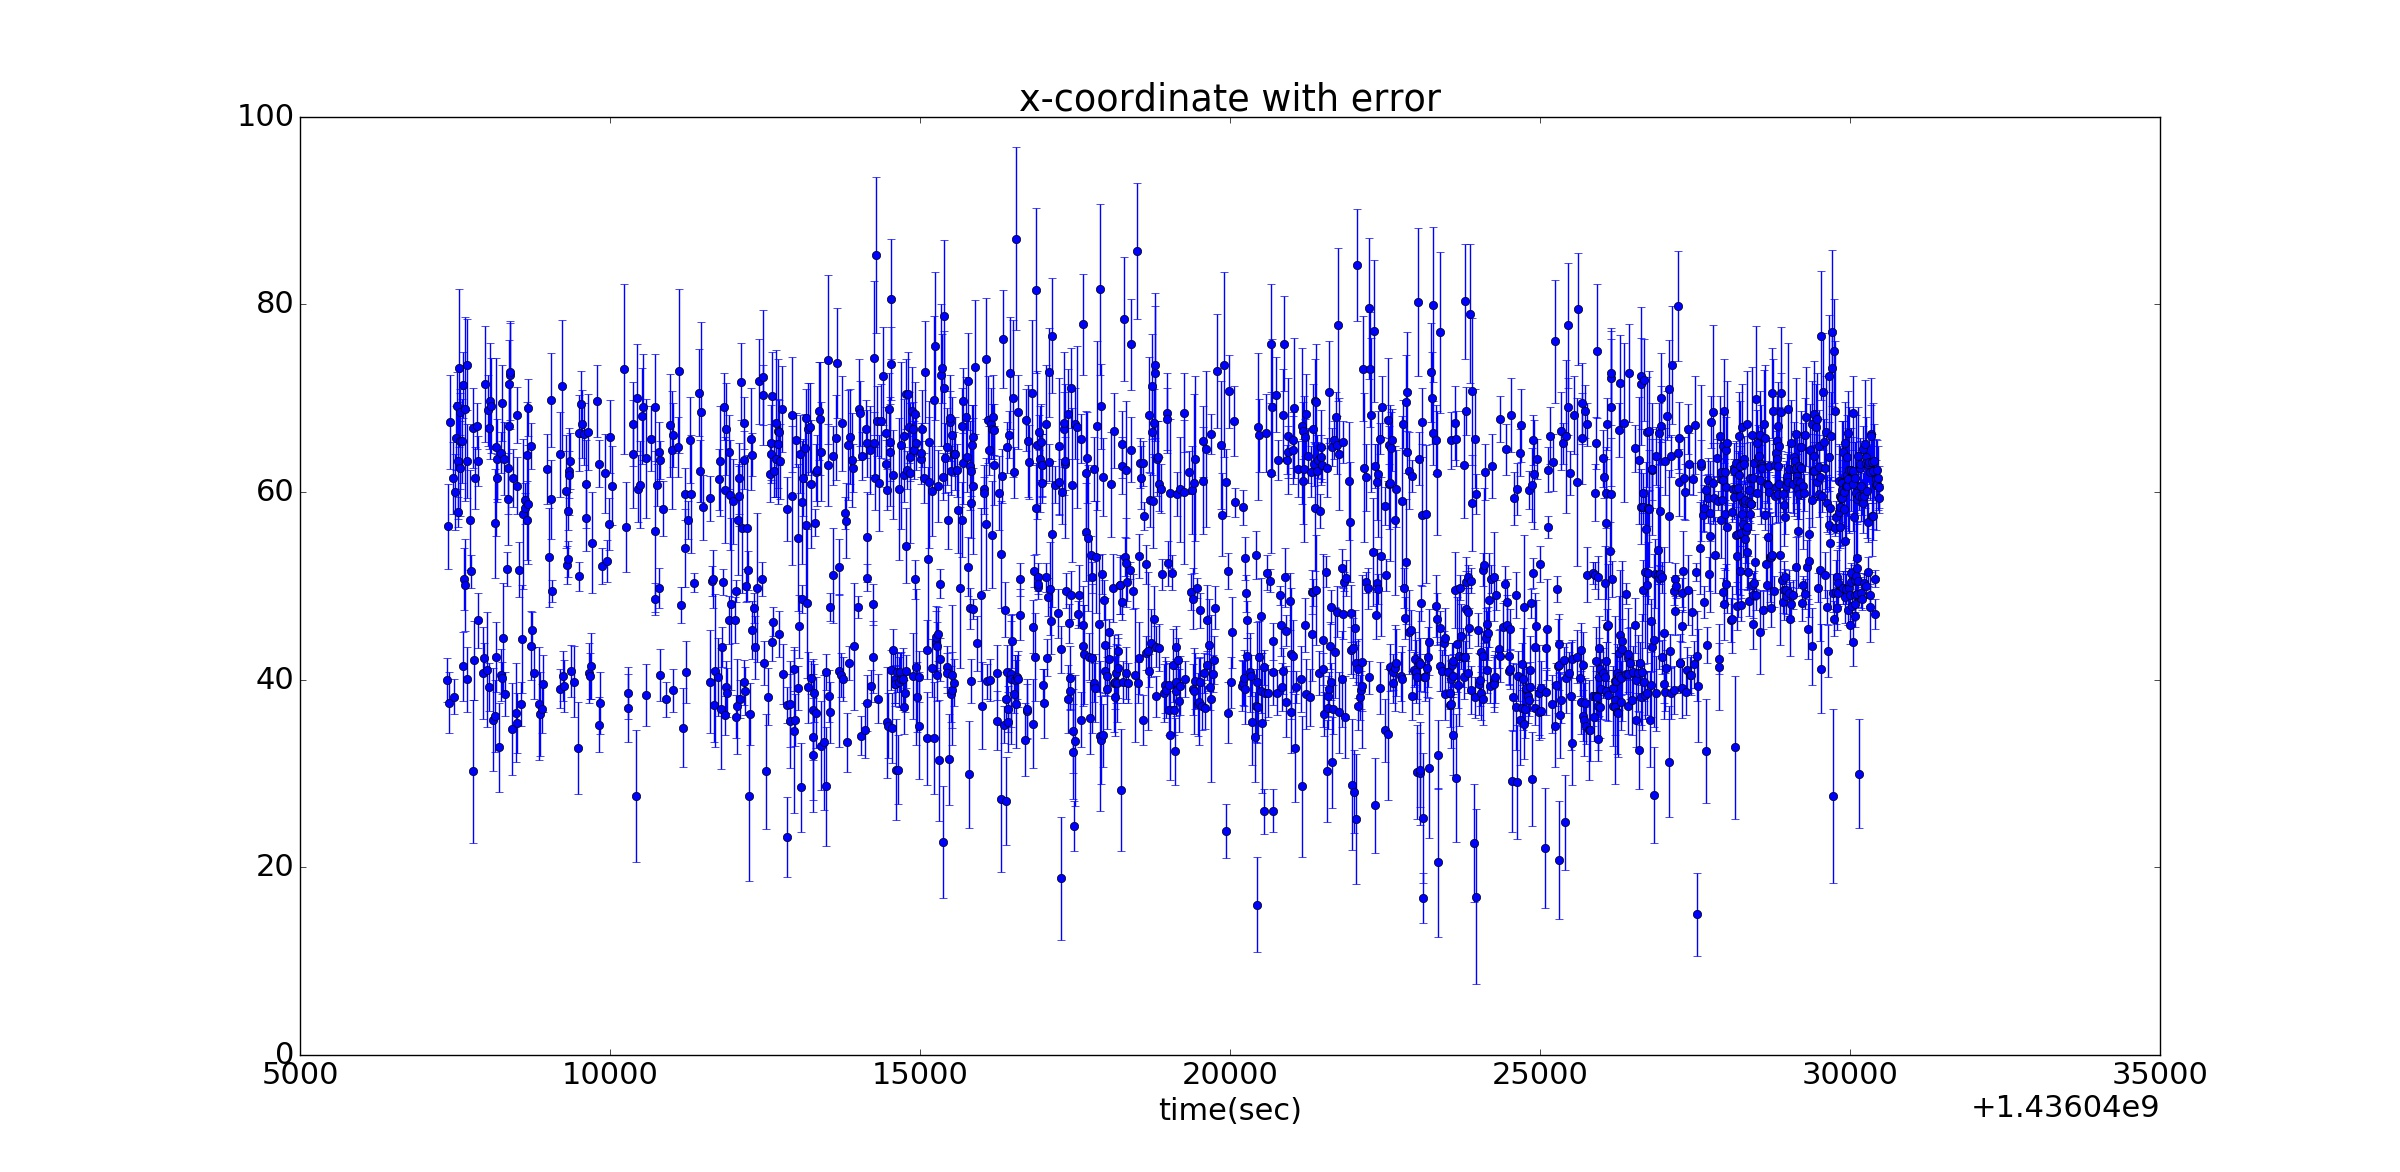
\includegraphics[width=120mm]{bimodal.jpg}
			\caption{Estimation of x-coordinate of a static MAC device through time with error}
			\label{fig:bimodal}
		\end{figure} 
	This figure shows the estimated x-coordinates in meters through time of a static MAC address that was persistent for 24 hours. Because we did not observe  bi-modal distributions in the signal strengths, the bi-modal distribution of the positions estimates can be explained by a "multiple local optima" situation. Namely, in a dense crowd, when optimizing the positioning of a MAC device, there can be multiple local optima that are equally good candidates. For example, consider Fig. \ref{fig:trilateration_problem} \footnote{Picture courtesy of http://math.stackexchange.com/questions/42537/trilateration-with-bounds}. \marginpar{change the position of the label and put units (meters)}In the center of every ring there is a Wi-Fi router, that has estimated signal strength to the MAC device with a certain error range. The error range is represented by the thickness of the ring. Then, there are two possible regions which are equally good candidates for the positioning of the MAC device, and those regions are the two darkest regions where all three rings overlap. Note that the problem can arise regardless of the thickness of the rings and the number of Wi-Fi routers. 	
	\begin{figure}[h!]
		\centering
		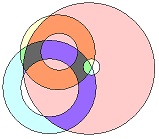
\includegraphics[width=40mm]{trilateration_problem.jpg}
		\caption{Trilateration can lead to multiple local optima}
		\label{fig:trilateration_problem}
	\end{figure}
	
	
\item {\it Issue 2: volatility of packet rates}. When a MAC device is connected to the Wi-Fi internet, it sends packets with a relatively stable and frequent rate. However, during concert hours, very few devices are actually connected to the internet. So, most of our estimations of positions come from signals that the device sends in a "probing" mode, i.e. while searching for a network. In this case the packet rate is quite volatile, ranging from a few seconds to a few minutes (citation?)\marginpar{add citation}. This means that when we make a snapshot of the MAC addresses visible in a certain moment, we are detecting a only a very small fraction of the MAC devices.   

\item {\it Issue 3: MAC address randomization}. Due to ever increasing privacy concerns and possibly other business reasons, starting from 2014, the Apple I-phones have introduced randomization of the MAC address when the device is in a probing mode (not connected to internet) (citation?)\marginpar{add citation}. This means that when the device switches from a probing to an online mode or vice versa, the MAC address suddenly changes and thus the device cannot be followed anymore. It is worth noting, however, that from the MAC address itself it can be determined whether the address is an original MAC address (non-randomized) or randomized. 
\end{enumerate}


\subsection{Crowd density estimation}

\subsubsection{Bimodal distributions of coordinates estimations: Creating statistical ensembles}


In order to deal with issue 1 from above, let us start with the following observation: we are not interested in the individual locations of the MAC devices, but rather in the density of the crowd. Also, we would  especially like to have more precise estimation when the density reaches a certain threshold, so that the crowd outside the dense region can be promptly navigated away from it. 
This situation (dense crowd), means that there is more blockage and absorption of signals from bodies. This leads to less precise estimation of the distance between a MAC device and a Wi-Fi router based on Wi-Fi signal strength, which means that the rings in e.g.  Fig.\ref{fig:trilateration_problem} would be even thicker. This exaggerates the effect of "bimodal" or even multi-modal distribution of position estimates. Thus, in a dense crowd, the best that we can derive from the positioning method for a MAC device is a probability distribution over all possible locations. For example, in the scenario in Fig. \ref{fig:trilateration_problem}, we can say that the MAC device is with a probability of 0.5 in the left grey region (region where all three rings overlap) and with a probability of 0.5 in the right grey region \footnote{In this example we assign the probabilities in a trivial way for the purpose of demonstrating our idea}. While this does not provide us with  very useful information about the location of the MAC device, if we apply the same reasoning for all MAC devices, and we add together the spatial probability density functions for all MAC devices, we end up with a spatial distribution of the crowd density. If we assume that the locations of the MAC devices are mutually independent, we can  apply directly the law of the large numbers and conclude that for a dense crowd the error of the estimation of the density per square meter will vanish. However, we cannot assume the mentioned independence, because people tend to go to concerts in groups. In this case, the variance of the estimation in the limiting case is equal to the average correlation between the locations. Nevertheless, we can safely assume that for a regular crowd at a concert the group size is relatively small compared to the whole crowd and thus the average correlation tends to zero as the number of people increases. Thus, the error of the estimation of the crowd density will in anyway diminish as the number of people grows. 

In what follows we formalize the discussion above. 
Let $\{mac_1, mac_2,...mac_n\}$ be all MAC devices detected at time $t$. Let $R$ be an arbitrary region from the stadium.  Let $X_i$ be a random variable defined by

$$X_i = 
\left\{
\begin{array}{ll}
1  & \mbox{if } mac_i \in R \\
0 & \mbox{if } mac_i \notin R
\end{array}
\right.  $$
Denote by $X$ the total number of devices in $R$ detected at time $t$. Clearly, $X=\sum_{i=1}^{n} X_i$.
Then $E(X)$, the expected value of $X$ is $$ E(X) = E(\sum_{i=1}^{n} X_i) = \sum_{i=1}^{n}E( X_i) = 
\sum_{i=1}^{n}(1\cdot Prob(mac_i \in R) + 0 \cdot Prob(mac_i \notin R)) = \sum_{i=1}^{n} Prob(mac_i \in R) ,$$
where by $Prob(mac_i \in R)$ we denote the probability that $mac_i$ is in the region R at time $t$.
We postpone the derivation of $Prob(mac_i \in R)$ a bit.  Instead, we first show that the variance of $X/n$, that is, the variance of the proportion of devices detected in $R$ out of all detected devices, diminishes when $n$ becomes large (note that the variance of $X$ in the limiting case is out of our interest because then $E(X)$ is potentially infinite). This suffices to show that our method of estimation of crowd density is theoretically sound, given the probabilities $Prob(mac_i \in R)$. We have

\begin{equation}\label{eq_Var}
Var(\frac{X}{n} ) =  Var(\frac{1}{n} \cdot \sum_{i=1}^{n} X_i) = \frac{1}{n^2} \cdot Var(\sum_{i=1}^{n} X_i) = \frac{1}{n^2} \cdot (\sum_{i=1}^{n} Var(X_i) + \sum_{i \not =  j}Cov(X_i,X_j))
\end{equation}


We can assume that there is an upper limit $\lambda$ of a number of people that go to a concert together (a group), that is, whose locations are correlated\footnote{Actually, when the crowd is so dense that people can not move freely anymore, the whole crowd becomes a "group" (as in the  Love Parade disaster) and all locations are correlated. But we aim to detect a high density with our method {\it before} this happens, to react preventively; otherwise, it is too late.}. Denote by $\kappa$ the maximal covariance between any $X_i$ and $X_j$ and let us write $i \sim j$ if and only if $i$ and $j$ are in the same group. 
Then, 
\begin{equation}\label{eq_covar}
\sum_{i \not =  j}Cov(X_i,X_j) = 2 \sum_{1\leq i <  j \leq n }Cov(X_i,X_j) =  2 \sum_{i,j: i \sim j }Cov(X_i,X_j)  \leq 2 n \cdot \frac{\lambda(\lambda - 1)}{2} \cdot\kappa = n  \kappa \lambda(\lambda - 1)
\end{equation} 
where the inequality holds because the maximal number of groups is $n$ and the maximal number of pairs $(i,j)$ in a group is $\lambda(\lambda-1)/2$.
Let $$\mu = \frac{1}{n}\sum_{i=1}^{n} Var(X_i),$$ that is, 
denote by $\mu$ the average variance of ${X_1, X_2, ..., X_n}$.  From \eqref{eq_Var} and \eqref{eq_covar} we have  

\begin{equation}
Var(\frac{X}{n} ) \leq \frac{1}{n^2}(n \mu + n  \kappa \lambda(\lambda - 1)) = \frac{1}{n}(\mu +  \kappa \lambda(\lambda - 1)), 
\end{equation}
which tends to $0$ when $n \rightarrow \infty$. Note that we have greatly overestimated the covariance with the inequation in \eqref{eq_covar}, which means that in practice the variance converges to $0$ much faster than as presented. 

Next, we can proceed with derivation of $Prob(mac_i) \in R$ for arbitrary $i$ in order to be able to evaluate $E(X)$, the estimated crowd density per region. 
   



\begin{comment}
To visualise the spatiotemporal behaviour of crowd density in real-time we dynamically generate heat maps along a moving time interval. The heat maps are generated through the statistical modeling of the positioning data. The generation of dynamic heat maps allows us to detect and locate hot-spots of density where crowd conditions reach critical values that could possibly lead to a disaster.
\end{comment}

The data provides us with a series of estimated positions of mobile devices, together with their corresponding values of measurement uncertainty (see Sec.\ref{sec:positioning}).

%The uncertainty values are determined by the co-variance matrix resulting from the chi-square fitting method.

From this data we wish to estimate the spatial probability distribution for an arbitrary MAC device $m$, along a moving time window.
So, our first step is to select from the data the estimated $N$ positions whose time stamps fall within a specified time interval $[t-\Delta t,t]$.
A natural way to construct a two-dimensional probability distribution would be to construct a histogram, by binning the positions and normalizing with $N$.
However, we also wish to preserve the uncertainty that corresponds to each estimated position.
Therefore, we first "smooth" each position into a bivariate Gaussian distribution (`bump'), using the uncertainty values ($\sigma_{x}$ and $\sigma_{y}$) provided by the data as standard deviations. Then, for  $m$ we construct a two-dimensional probability density function (p.d.f.) by adding up these bumps, and  dividing the sum by $N$.\marginpar{make viz. smooth and not dark}. (In Fig. \ref{fig:smoothing} we show the result of smoothing a histogram of the device discussed in Fig.\ref{fig:bimodal}.) %For example, 

\begin{figure}[h!]
	\centering
	\begin{subfigure}{.4\textwidth}
		\centering
		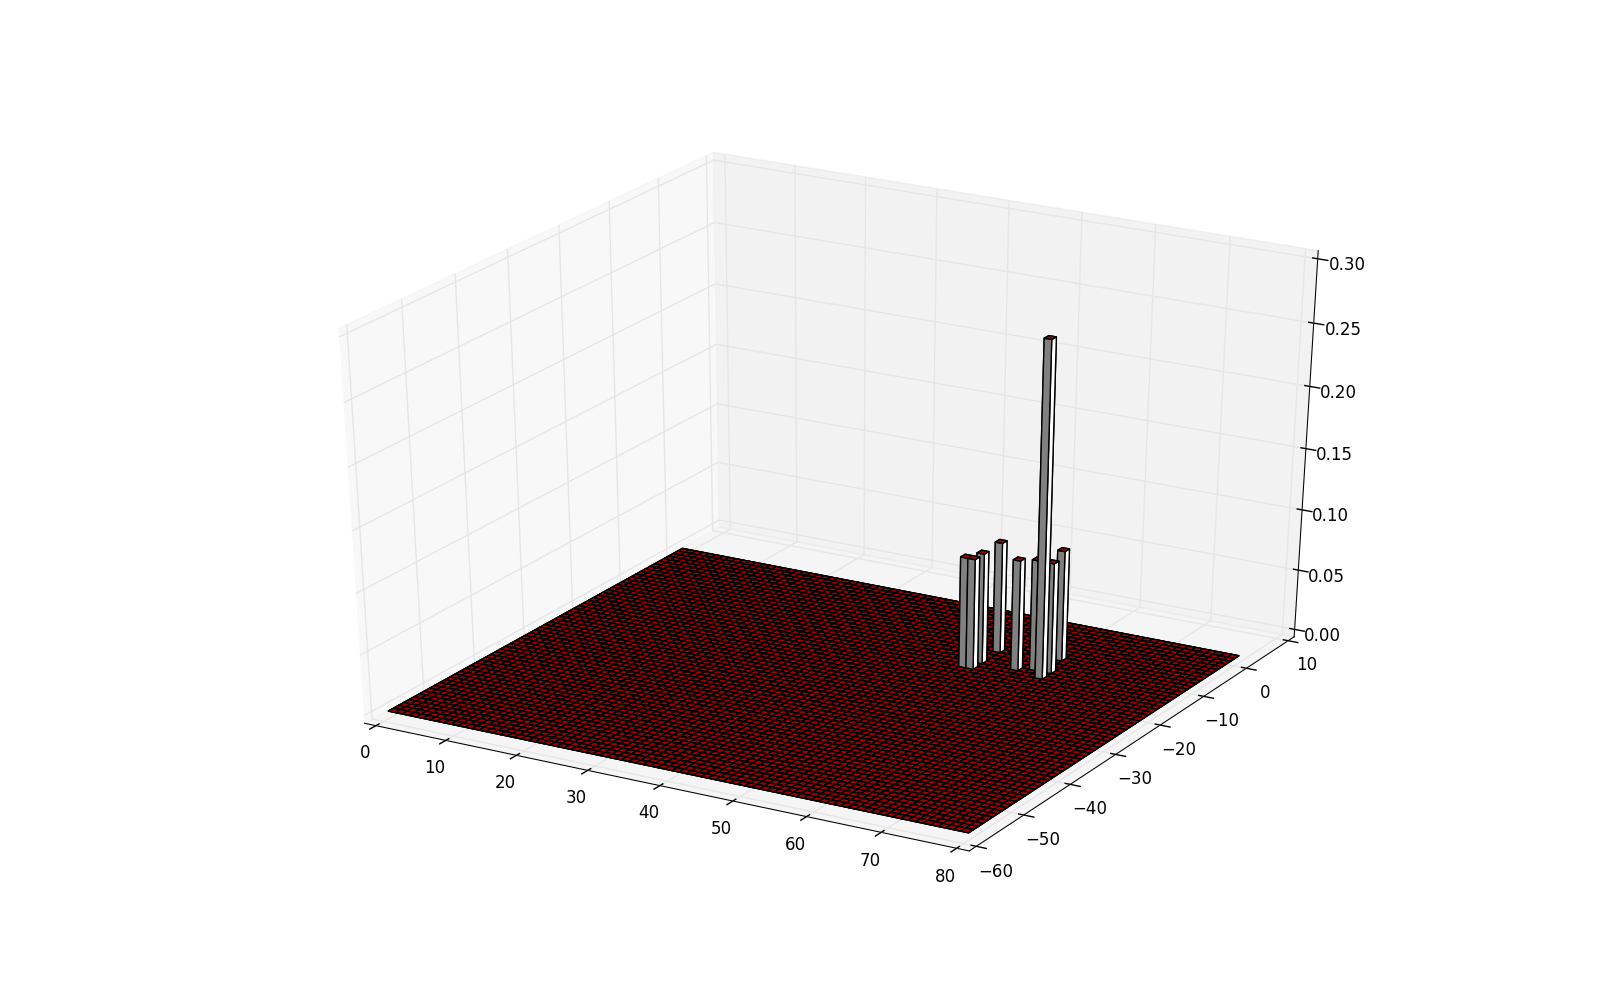
\includegraphics[width=1\linewidth]{non-smoothed-histo.png}
		%\caption{1a}
		%\label{fig:sfig1}
	\end{subfigure}%
	\begin{subfigure}{.4\textwidth}
		\centering
		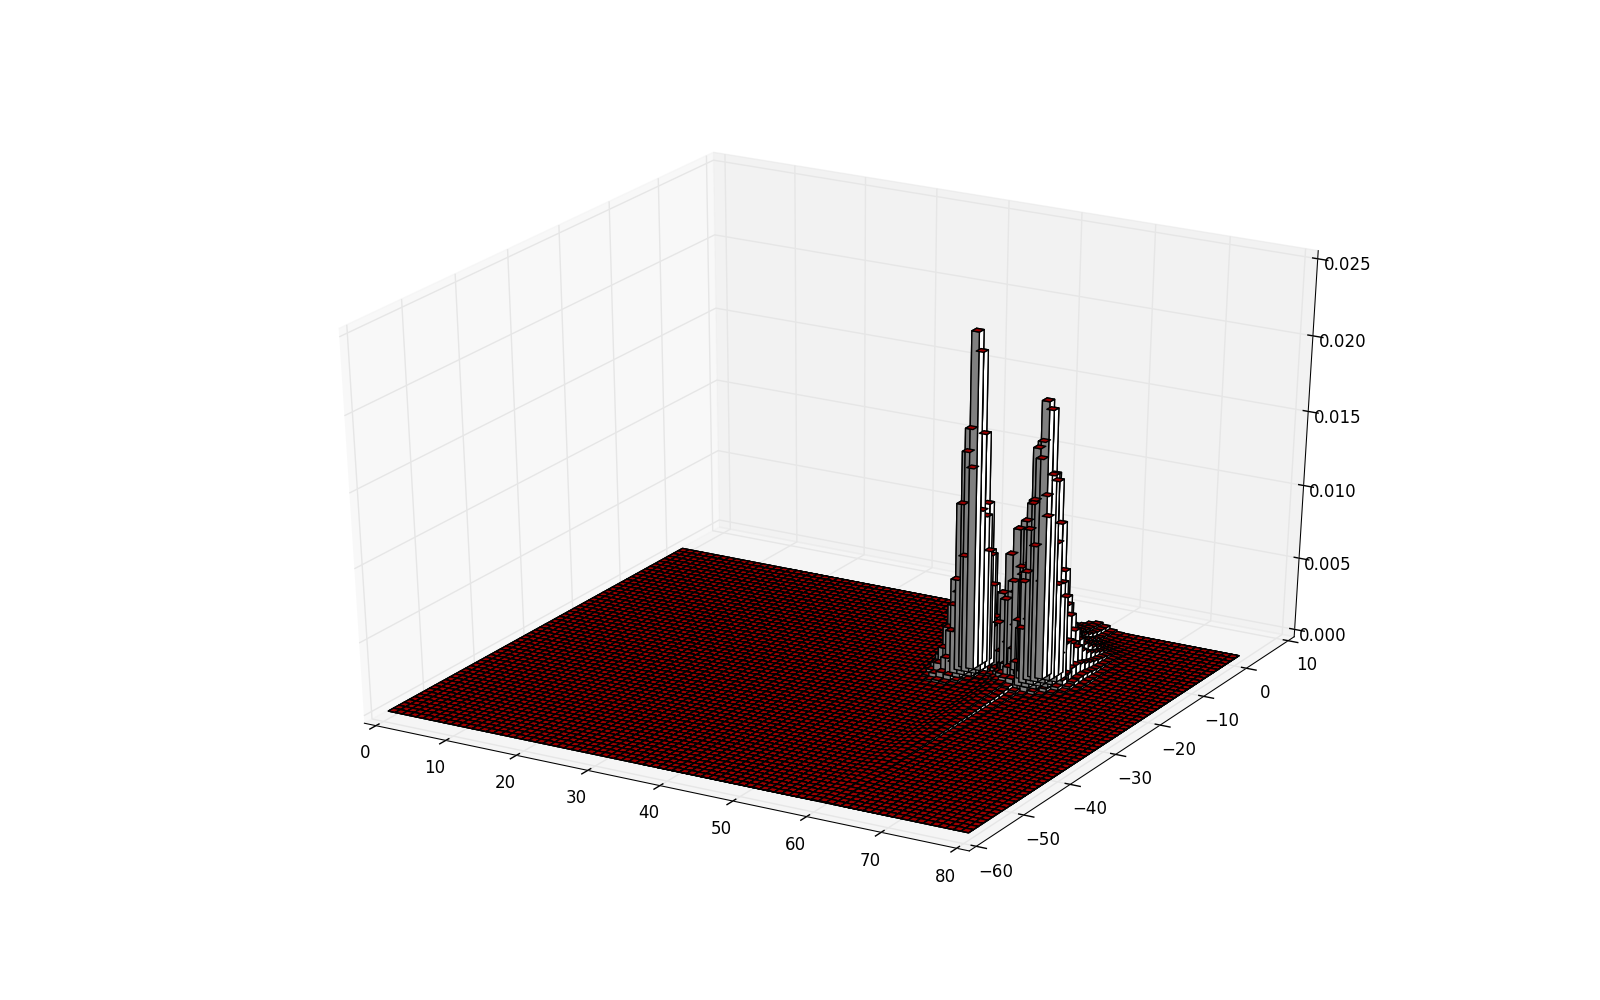
\includegraphics[width=1\linewidth]{smoothed-histo.png}
		%\caption{1b}
		%\label{fig:sfig2}
	\end{subfigure}
	\caption{Smoothing a histogram with Gaussian kernels. Left: Original histogram. Right: The smoothed histogram.}
	\label{fig:smoothing}
\end{figure}


The implementation of our method is similar to that of kernel density estimation \cite{scott}\cite{silverman}.
In our case the amount of smoothing is variable and determined by the measurement uncertainty values $\sigma_{x}$ and $\sigma_{y}$.
The p.d.f.  for a mobile device with an address  $m$ at a location $(x,y)$ is defined by

\begin{equation}
\hat{f}_{m}(x,y)=\frac{1}{N}\sum_{i=1}^{N}K((x-x_{i}),\sigma_{x}) K((y-y_{i}),\sigma_{y})
\label{kde}
\end{equation}
where the kernel function $K$ is given by
\begin{equation}
K(u,\sigma)=\frac{1}{\sigma\sqrt{2\pi}}\exp(-\frac{u^2}{2\sigma^2})
\end{equation}
The final crowd density estimation is given by
\begin{equation}
\hat{f}_{T}(x,y)=\sum_{m}\hat{f}_{m}(x,y)
\label{total}
\end{equation}
To finish our  discussion, in order to evaluate $Prob(mac_i) \in R$ we need to integrate $\hat{f}_{m}(x,y)$ for $(x,y) \in R$. 

Note that so far we assumed that in every time window there is at least one estimate for every MAC address ever detected. In what follows we explain how we capture the cases when this assumption does not hold. 

\begin{comment}
\subsection{Real-time data analysis}

To process positioning data in real-time during events, we consider data within a specific moving time window.
To take in account that visitors are moving, we subdivide the time window in multiple sub-windows and attach more weight to measurements in later sub-windows. The weighting scheme is given by

\begin{equation}
\hat{d}(X,t)=\frac{w_{1}\hat{f}(X,t_{1})+w_{2}\hat{f}(X,t_{2})+...+w_{m}\hat{f}(X,t_{m})}{w_{1}N_{1}+w_{2}N_{2}+...+w_{m}N_{m}}
\end{equation}

\noindent where $\hat{f}(X,t)$ is the non-normalized sum of smoothed counts ($N\times\hat{d}(X,t)$) in Equation \ref{kde}, $w_{k}$ is the weight value given to sub-window $k$, and $m$ is the number of sub-windows.
\end{comment}

\subsubsection{Volatility of packet rates: Applying "conservation of mass" principle }

(Needs to be finished.)
To address the second issue, {\it Volatility of packet rates}, we ensure that we do not forget about the MAC devices that were not observed in the last time window. In fact, for every MAC device that was ever observed, until it has been observed again we maintain the old probability distribution, too. Over time this probability distribution turns gradually into a uniform by smoothing it every epoch with a Gaussian kernel (see Fig. \ref{fig:uniform} for an example). The size of the kernel changes over time and is related to the maximal speed that the MAC device can have under the current density distribution of the crowd. In other words, we assume a Brownian motion of the MAC device, where the speed is limited by the maximal speed of a pedestrian under the current crowd conditions (cite paper Johansson et al). When the MAC device is observed again, its old probability distribution is simply overwritten by the probability distribution that is computed as above.\marginpar{ref.  picture}

%\begin{figure}[h!]
%	\begin{subfigure}
%	\centering
%	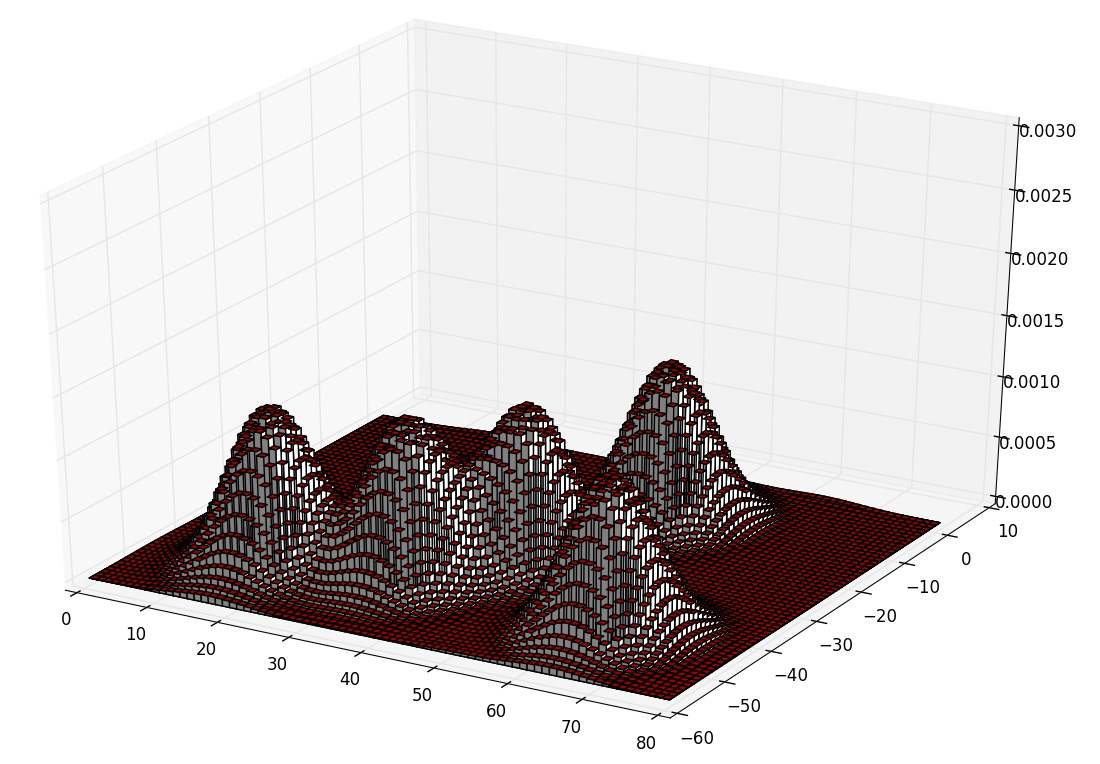
\includegraphics[width=60mm]{brownian-smoothing-0002.png}
%	\end{subfigure}
%	\begin{subfigure}
%	\centering
%	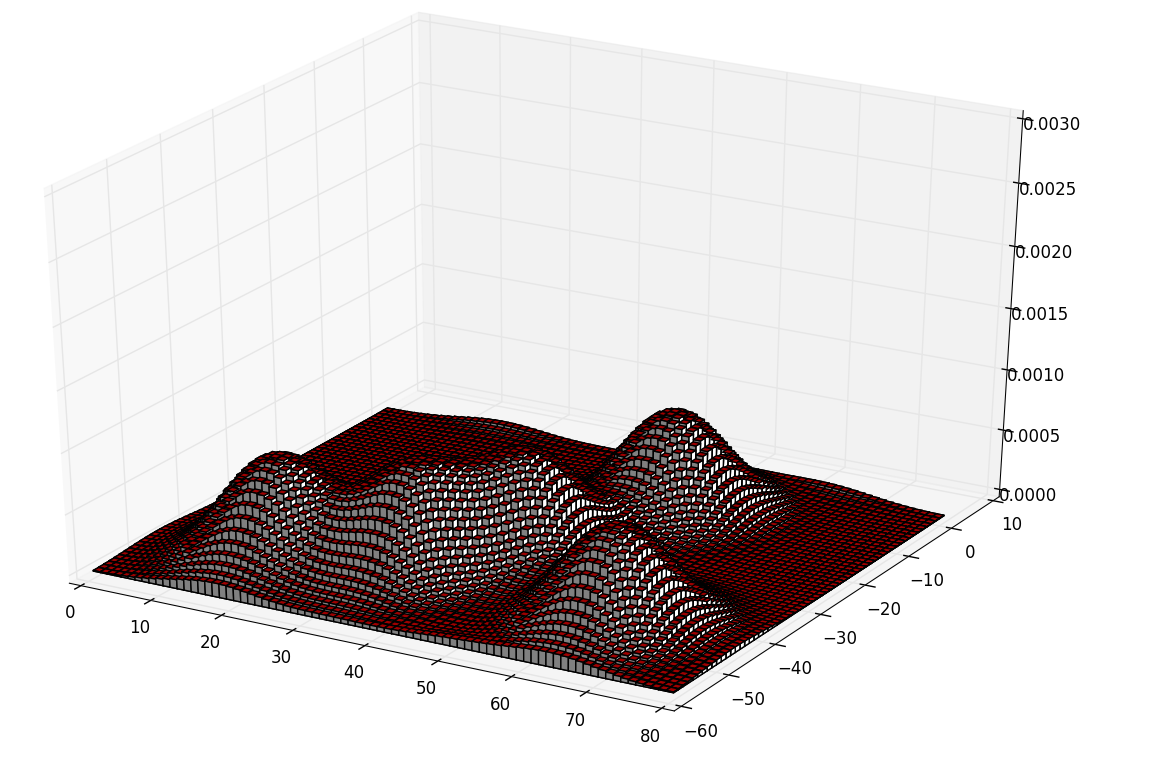
\includegraphics[width=60mm]{brownian-smoothing-0004.png}
%    \end{subfigure}
%	\begin{subfigure}
%	\centering	
%	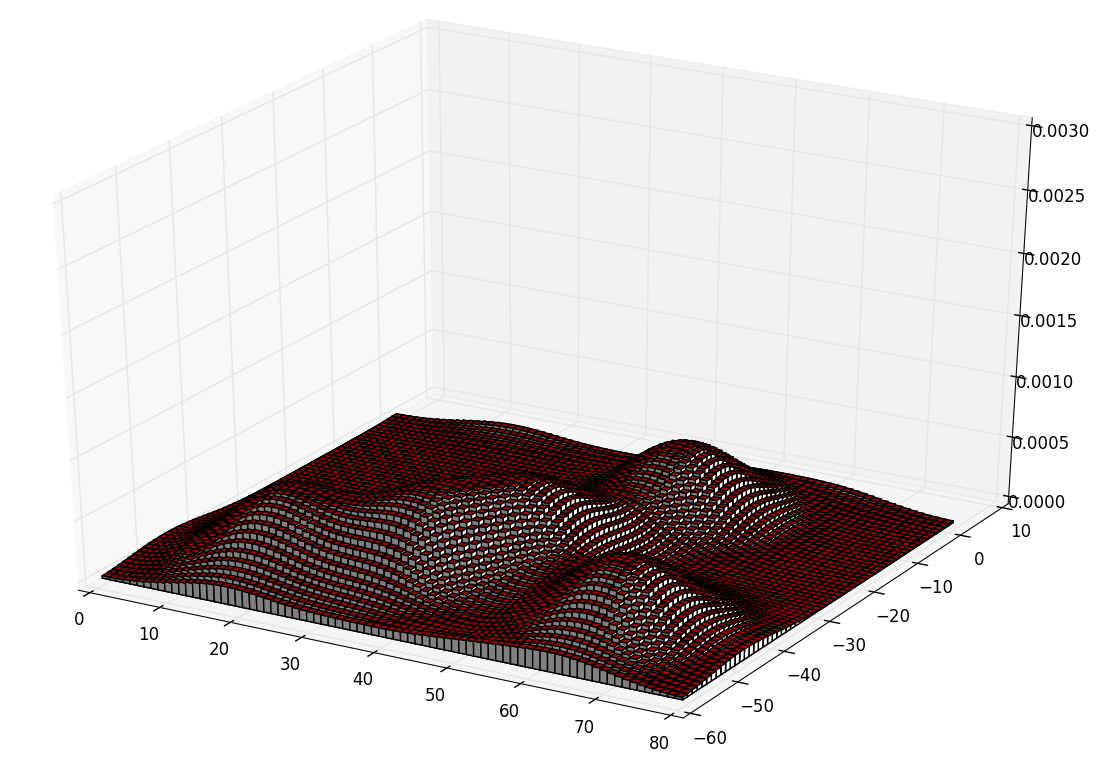
\includegraphics[width=60mm]{brownian-smoothing-0006.png}
%	\end{subfigure}	
%	\caption{Turning a distribution gradually into uniform}
%	\label{fig:uniform}		
%\end{figure}

\begin{figure}[h!]
	\begin{subfigure}{.3\textwidth}
		\centering
		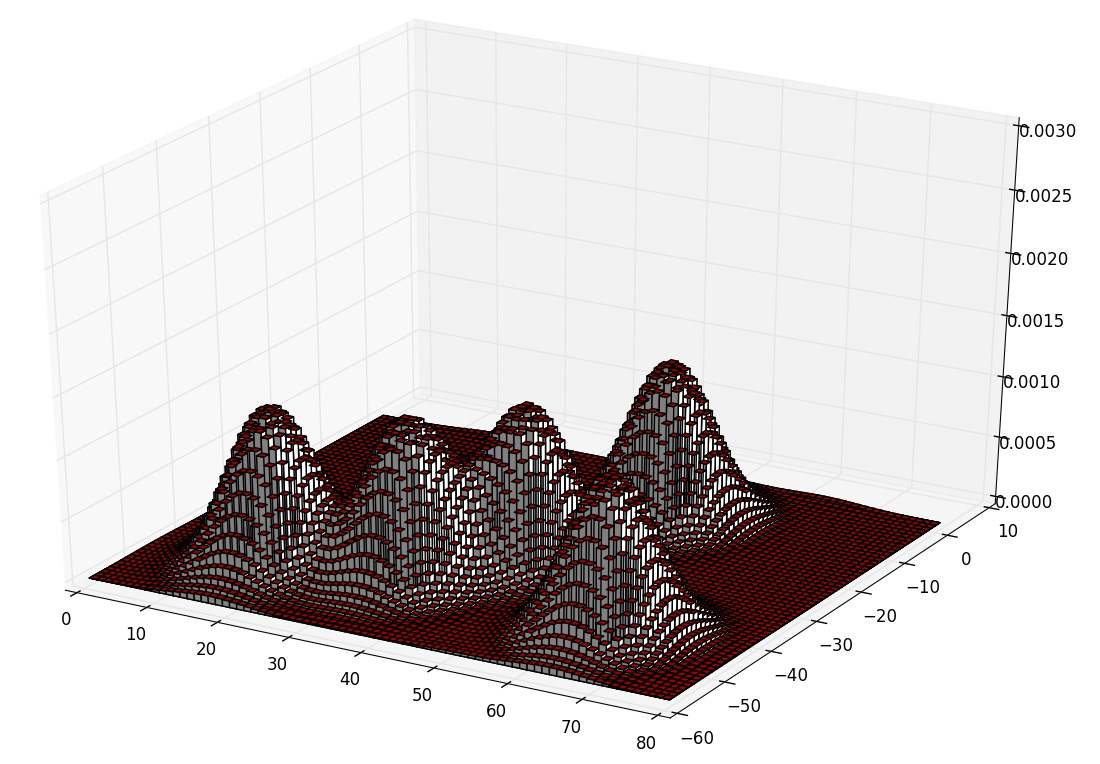
\includegraphics[width=1\linewidth]{brownian-smoothing-0002.png}
		%\caption{1a}
		%\label{fig:sfig1}
	\end{subfigure}%
	\begin{subfigure}{.3\textwidth}
		\centering
		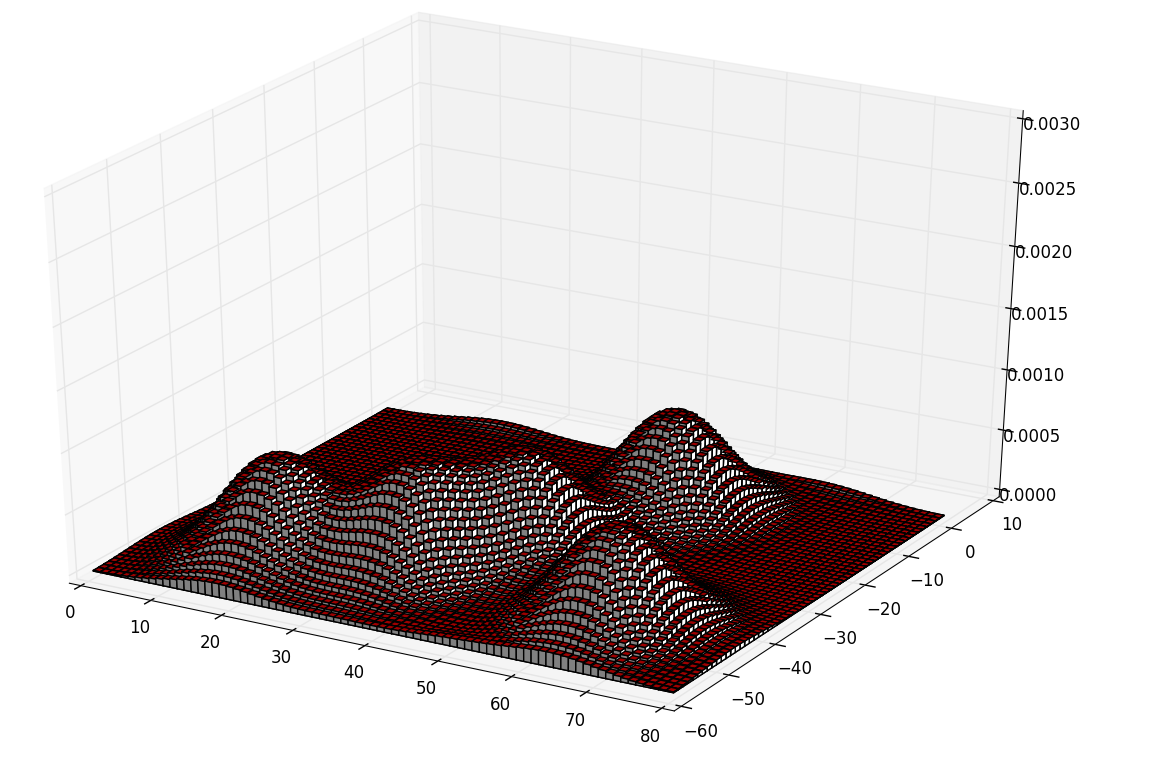
\includegraphics[width=1\linewidth]{brownian-smoothing-0004.png}
		%\caption{1b}
		%\label{fig:sfig2}
	\end{subfigure}
	\begin{subfigure}{.3\textwidth}
		\centering
		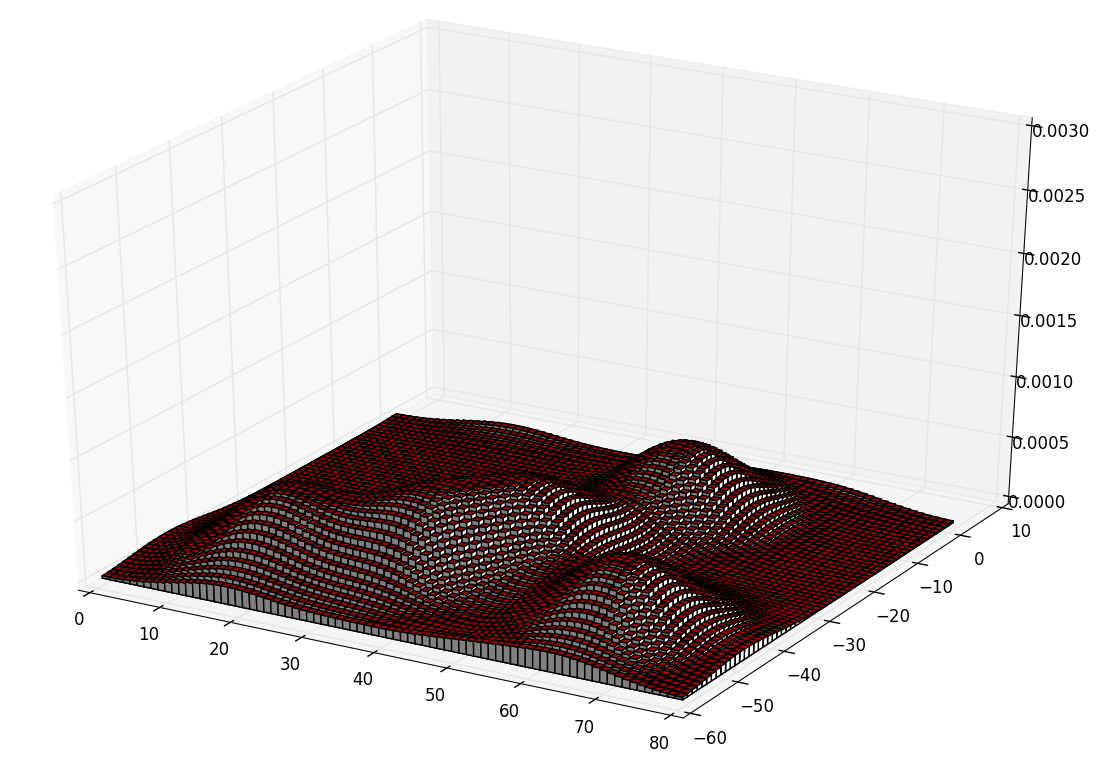
\includegraphics[width=1\linewidth]{brownian-smoothing-0006.png}
		%\caption{1c}
		%\label{fig:sfig3}
	\end{subfigure}
	\caption{Turning a distribution gradually into uniform}
	\label{fig:uniform}
\end{figure}

Formally, for the epochs during which a mobile device is not detected we assume Brownian motion (without drift), which is defined by
% had to change X to B because I used X for the random variables above. Sorry.
\begin{equation}
\text{d}B(t)=\sigma\text{d}W(t)
\end{equation}
where $W(t)$ is a Wiener process. The density function $f(t,x)$ of the displacement of $X$ in the time interval $[0,t]$ is known, and is a normal distribution with mean $B(0)$ and variance
\begin{equation}
\text{Var(\textit{B(t)})}=\sigma^{2}t
\end{equation}
Thus, in case we have no new observations, we smooth the density estimate from the previous epoch by convolution with the normal density function. 
The variance is determined by the length $t$ of the time interval, and the walking speed of pedestrians.
[Optional: We relate $\sigma^2$ to the walking speed of pedestrians as defined by]
\begin{equation}
\sigma^2=\frac{(\Delta B)^2}{\Delta t}
\end{equation}
The walking speed of pedestrians can be related to the local crowd density via the so-called \textit{Fundamental Diagram}. 
The fundamental diagram generally states that walking speed of pedestrians is a decreasing function of the local crowd density [(Weidman 1992)].
The fundamental diagram function has been the subject of extensive study [examples].
Although all these studies agree on the decreasing form of the function, empirical studies in different countries and cultures have resulted in different forms and parameters values.

Here we use the fundamental diagram as provided by ... [?]
\marginpar{add rescaling to include information that all visitors are still inside the stadium }


\subsubsection{MAC address randomization: using Big data again}

To address the last issue, {\it MAC address randomization}, we rely once again on the fact that we have a lot of data. Namely, we know from the structure of the MAC address whether it has been randomized or not. Figure \ref{fig:randomized} shows the ratio between randomized and non-randomized addresses observed per minute from midnight until 6:00 am. We can see that it is quite stable through time; in fact, the Pearson correlation coefficient between the time series of randomized and non-randomized addresses is 0.88. 

\begin{figure}[h!]
	\centering
	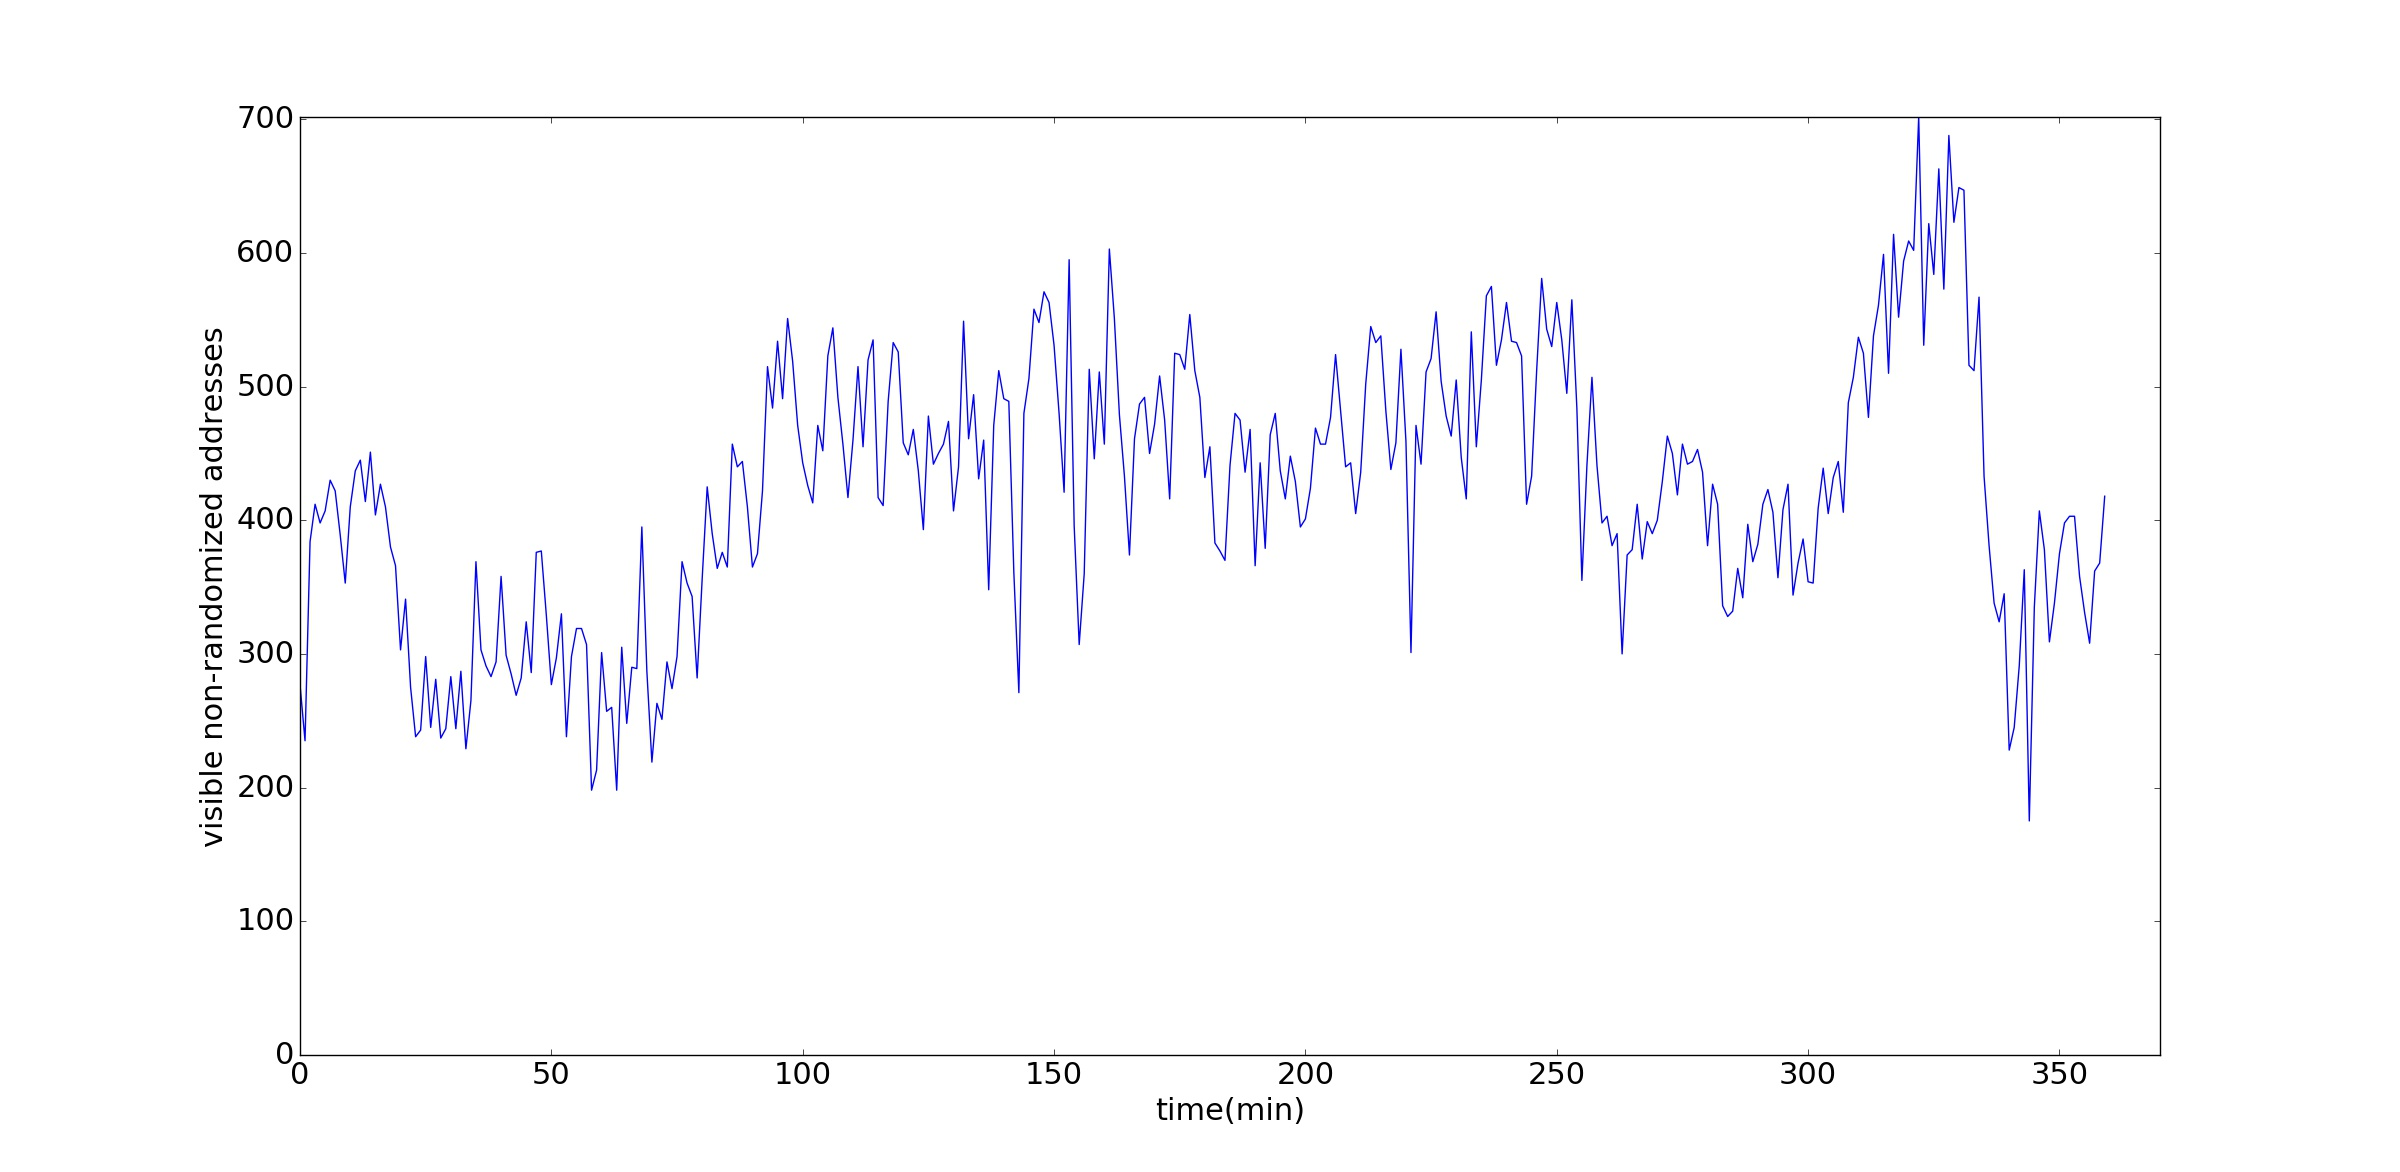
\includegraphics[width=130mm]{nonrandomized.jpeg}
	\caption{Non-randomized addresses observed per minute}
	\label{fig:nonrandomizedadresses}
\end{figure} 
\begin{figure}[h!]
	\centering
	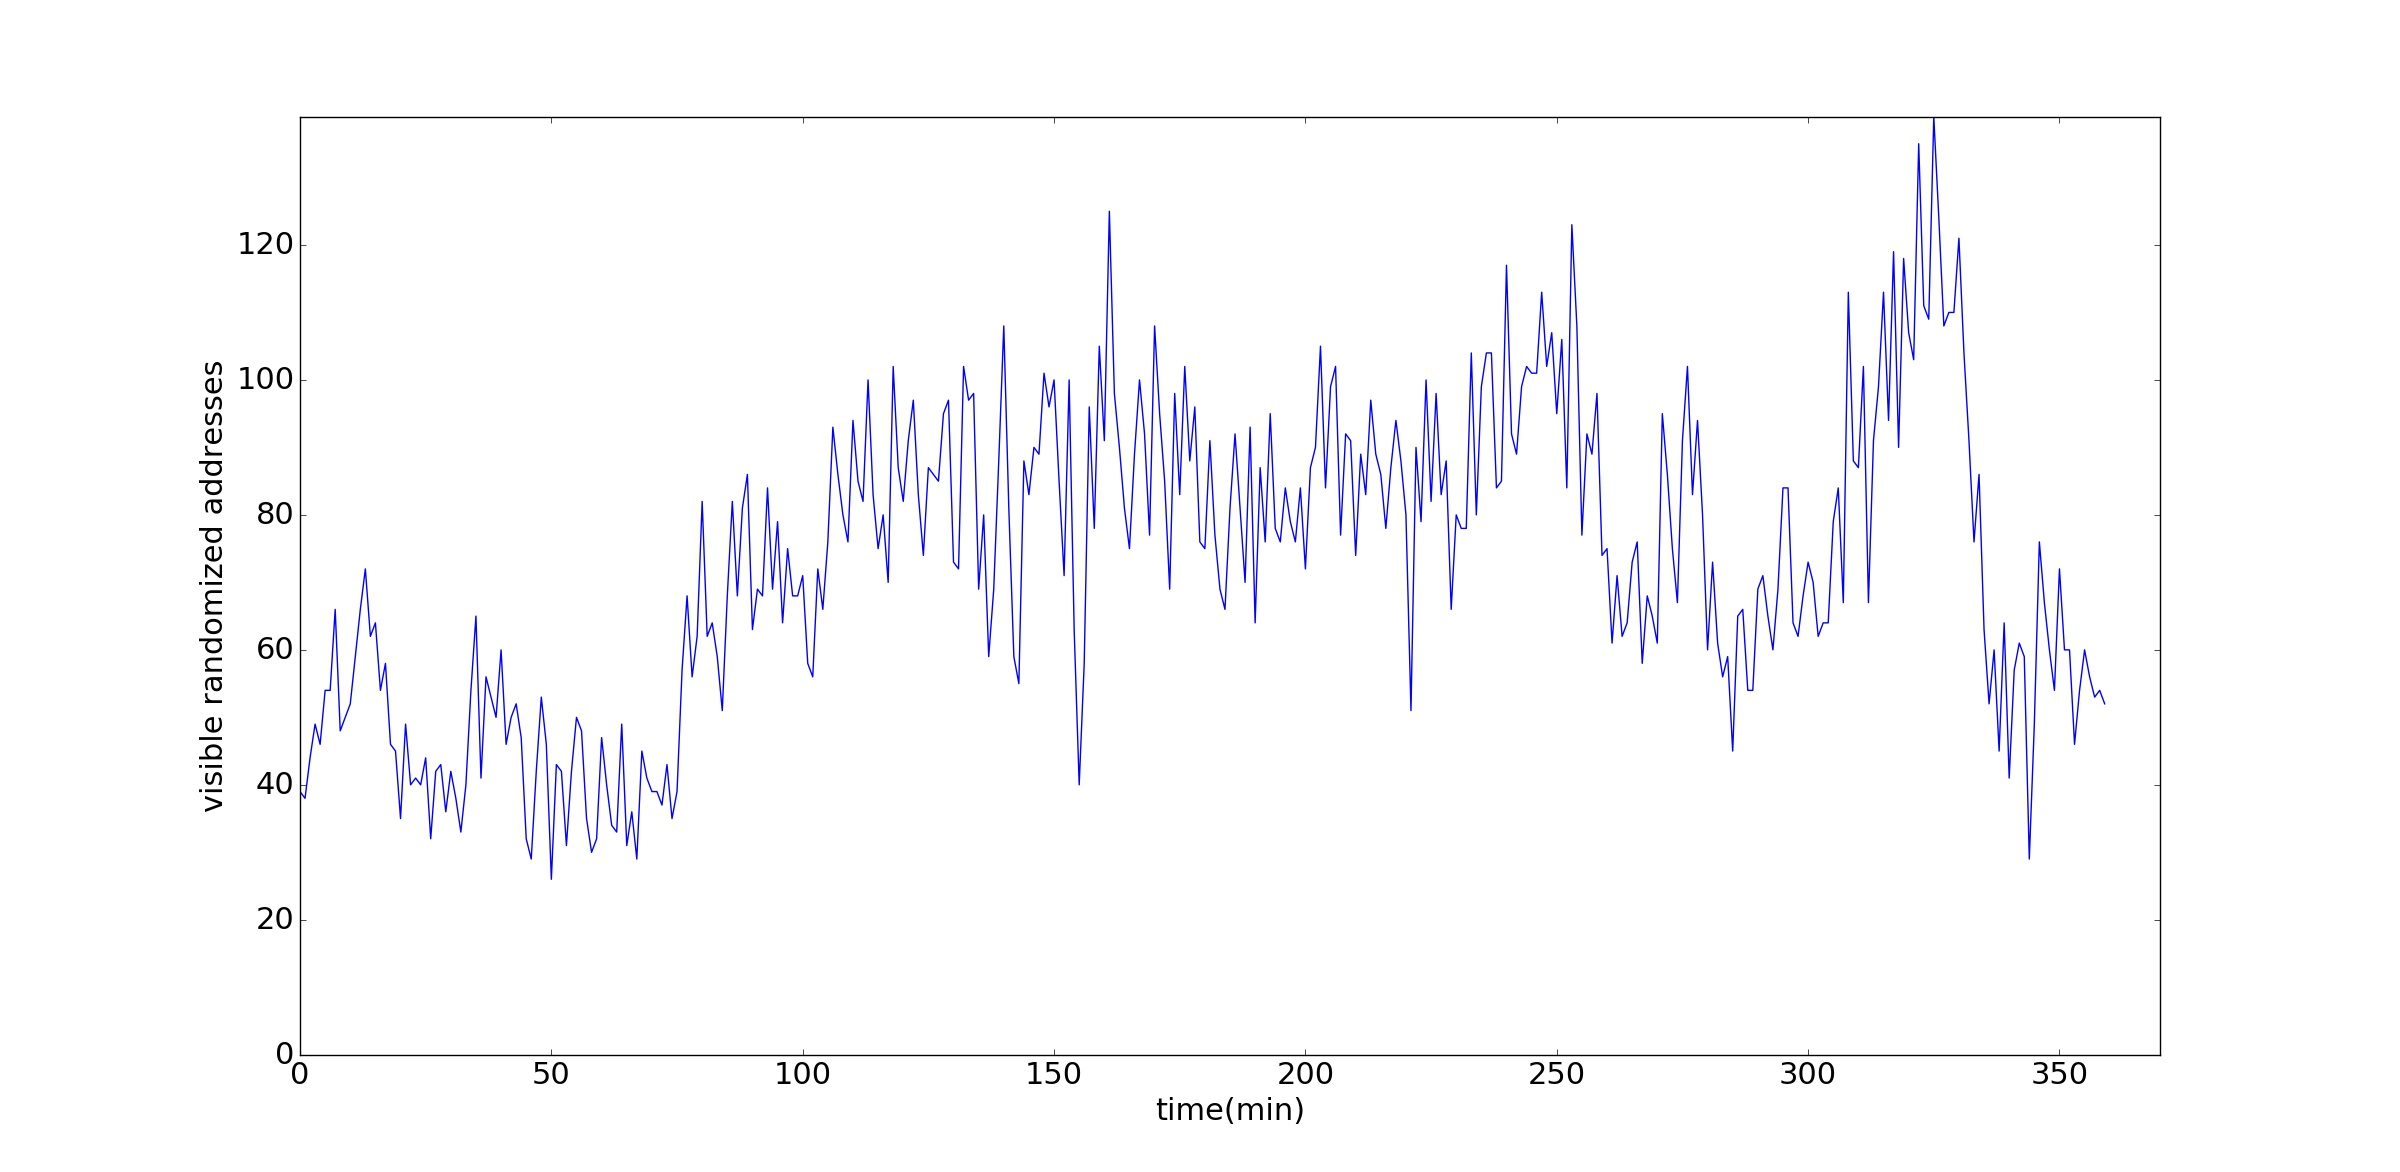
\includegraphics[width=130mm]{randomized.jpeg}
	\caption{Randomized addresses observed per minute}
	\label{fig:randomizedaddresses}
\end{figure} 
\begin{figure}[h!]
	\centering
	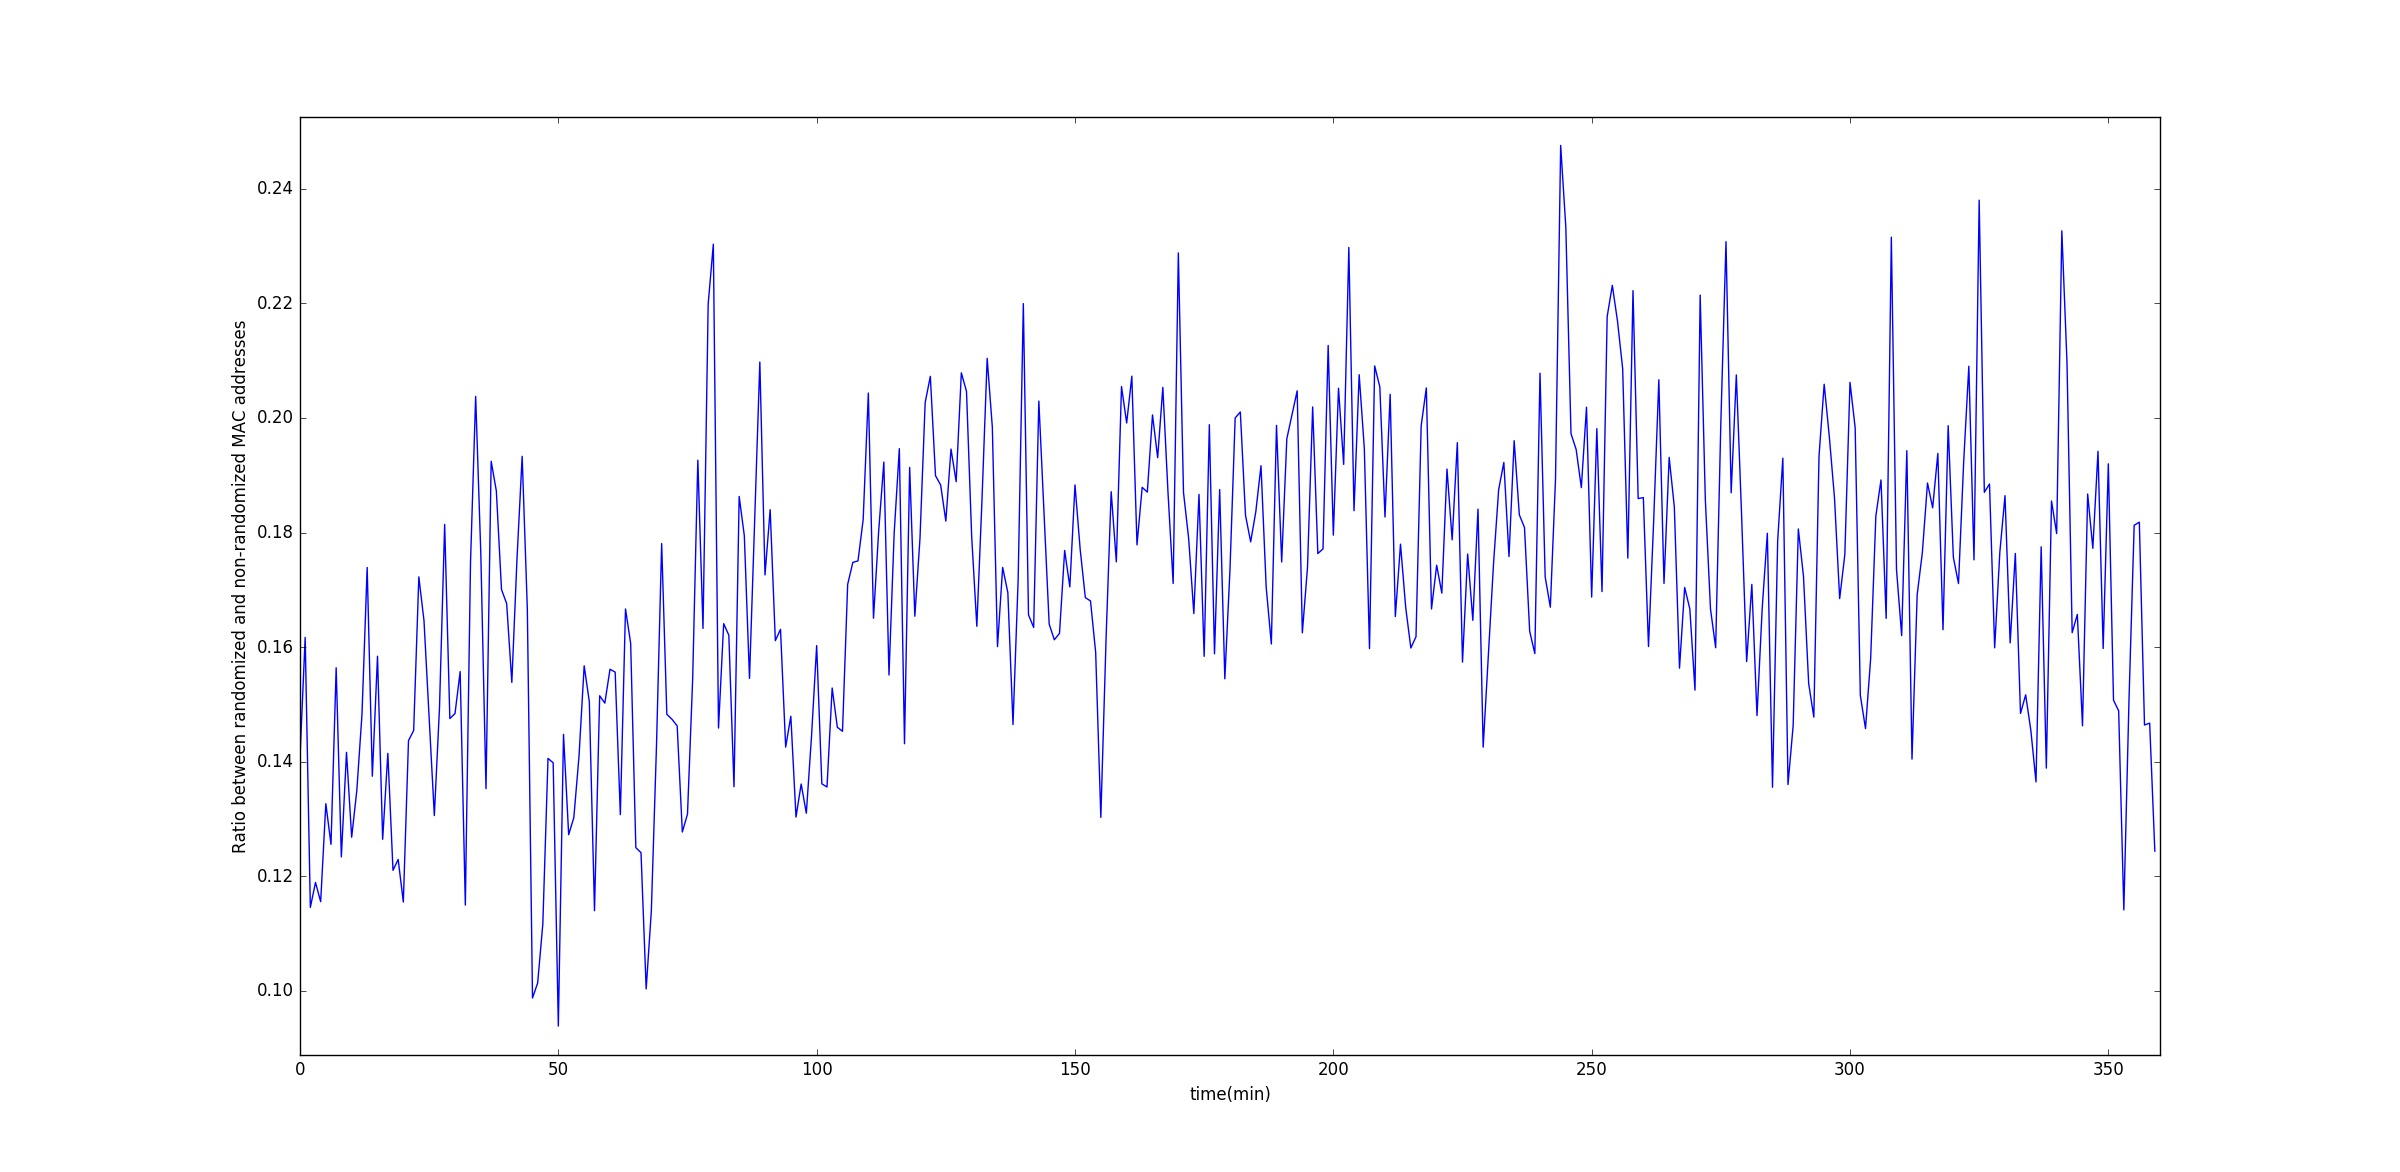
\includegraphics[width=130mm]{RatioRandNonrand.jpeg}
	\caption{Ratio between randomized and non-randomized addresses observed per minute}
	\label{fig:randomized}
\end{figure} 

\noindent Thus, when estimating crowd density, we ignore the MAC devices that have a randomized address and at the end we multiply the crowd density by 1.225, to account for the ignored MAC devices. We choose factor 1.225 to allow for a safety margin: in the peaks of the graph in Fig. \ref{fig:randomized} the values are 0.225, and we would rather overestimate than underestimate the crowd density. \marginpar{in general: calculate it automatically, with a confidence interval}
Note that this ratio should be re-computed periodically, to account for the changing conditions at the smart phones market. 
\marginpar{mention the absolute numbers, or give graphs}



\section{Validation}\label{sec:validation}
To be done.
Hopefully with official videos from the organizational team of  Sensation 2015 Amsterdam White.
Note that by validation we mean more of calibration. In general the approach is theoretically valid, which we show in Sec.\ref{sec:density}.2.1, but we are using parameters in the model that need to be calibrated. We need independent data sets (videos) for calibration and testing, to avoid overfitting. Also the paremeters should be as much as possible initially optimized from the Wi-Fi data itself and from theory.

\section{Related work}\label{sec:relatedwork}
In progress. 

In the Introduction we mentioned the benefits of using smart phones based over video-based approach for density estimation of indoor concerts crowd; in fact, it is our opinion that the two approaches complement each other and in the future we plan to integrate both techniques in real time. Thus, in this section we are going to focus on previous work that estimates crowd density using wireless technologies. 

\cite{weppner:1} estimate crowd densities by distributing volunteers in the crowd, who are carrying smart phones scanning for Bluetooth devices. They then use statistics to combine the different measurements in space and time. They improve their method from mere counting to more advanced statistical analysis in \cite{weppner:2}, by using relative features that are more robust
against statistical variations of the number of devices. The features include 
the average speed of scanning devices, the average bluetooth signal strength and its variance, etc.

%Wirz \textit{et al.} (2012) \cite{wirz:1} infer crowd density from GPS location traces of people who use an App during the 2011 Lord Mayor Show in London. They visualize the data in real-time, and generate heat maps (dynamically) using the kernel density estimation (KDE) method. 
In  \cite{wirz:2} the authors follow a participatory sensing approach in which pedestrians share their locations on
a voluntary basis. Since  only a fraction of
all pedestrians share location information, they present a methodology to infer the crowd density from their walking speed, by inverting the formula for estimating maximal pedestrian speed given a crowd density, presented in \cite{Johannsson}. Note that in our case study the visitors of the concerts with a stage are mostly static without intention to reach a destination, so this technique cannot be directly applied. 


%The Gaussian weight function used in (Wirz \textit{et al.} 2012; 2013) \cite{wirz:1}\cite{wirz:2} is introduced in Helbing \textit{et al.} (2007) \cite{helbing:1} to estimate local densities in an area captured by video cameras during the Hajj in Mina/Makkah in 1426H on January 12, 2006.\\

A number of studies use Bluetooth to estimate crowd densities at a wide range of places and events.
In these studies the position of a mobile phone is approximated to the location of the sensor by which it is detected.

Schauer \textit{et al.} (2014) \cite{schauer:1} count unique MAC devices detected by two sensors (nodes) at both sides (public and security) of a security check inside a major German airport, to estimate pedestrian densities and pedestrian flow. They consider time information, to determine the direction of a person's movement, and at least one RSSI value, to reduce the number of false positives in case devices are captured by both sensors. They compare Bluetooth and Wi-Fi based methods, and compare their methods to a known ground truth provided by the number of security checks.

Versichele \textit{et al.} (2012) \cite{versichele:1} use Bluetooth scanners at strategic locations during the 10-day Ghent Festivities, to analyze spatio-temporal dynamics of pedestrians. 

Yoshimura \textit{et al.} (2016) \cite{yoshimura:1} use Bluetooth detection to analyze visitors' behavior at the Louvre museum in Paris.

Delafontaine \textit{et al.} (2012) \cite{delafontaine:1} use a similar approach (of Bluetooth tracking) and apply (genetic) sequence alignment methods to analyze the resulting data which consists of different sequences of sensors (nodes) for detected mobile devices.



%In Weppner \textit{et al.} (2014) \cite{weppner:2} similar methods are applied to a city-wide festival in Zurich 2013, now supported by GPS data.

Finally, none of the mentioned work uses our approach of modeling the position of an individual as a probability distribution; our method is designed to attack the problem of having a dense crowd; we are not interested in precise estimations for freely moving crowds; rather, we are interested in obtaining precise estimation when the  concert crowds is dense and static...


\section{Conclusion}\label{sec:conclusion}
To be done. 
Sonja:Mention somewhere that in the documentary of the LP disaster people were raising their phones up to look for a way out. (which is good , less blockage of signals)




Future work: include map of the venue in the calculations, perhaps not both dark  regions in \ref{fig:trilateration_problem} are accessible by people!

Also future work: the speed in the brownian motion should depend on the local crowd density, rather than on the average crowd density.

\bibliography{references}
\bibliographystyle{plain}

\end{document}